\chapter{算法实现}
本章,我们将从判决预测、关键词抽取、类案搜索等模块来详细介绍项目中用到的算法模型。在模型中,我们统一使用了THULAC进行中文分词,我们使用的词向量是利用FastText模型,在大规模的法律文书语料库上进行的预训练,我们采用的词向量维度为200维。

对于每一个模块,我们将分别从任务的描述定义、算法的创新点、算法模型细节三个方面来进行详细阐述。


\section{判决预测}
\subsection{任务描述}
在该模块中,我们主要实现了案件的罪名及案由预测、相关法条推荐、刑事案件刑期预测、相关判案要素预测等功能。

输入一段文本形式的案情描述,模型通过阅读文本获取文本中蕴含的语义信息,将案情映射到一个高维向量空间中,得到一个包含有文本信息的文章向量,再根据不同的任务,将文章向量喂给不同的输出层获得不同的分类结果。

\subsection{创新点}
我们将上述所有功能归纳为文本分类问题,通过观察,上述任务之间有很强的前后依赖关系,例如,相关法条推荐结果往往与罪名及案由预测结果高度相关。并且,根据法学领域从业人员介绍,在实际判案时,大家首先会判断案情中的相关要素,并根据要素判断结果来决定最后的案件的判决。因此,我们有以下创新来提升各个任务的效果:

1)	在多任务学习(multi-task learning)中提出了一个新的架构,充分利用各个任务之间的依赖关系来共同提升多个任务的预测效果。

2)	模拟法官判案过程,提出判断案件判案要素作为中间任务,来大幅提升相关任务的效果。

\begin{figure*}[ht]
    \centering
    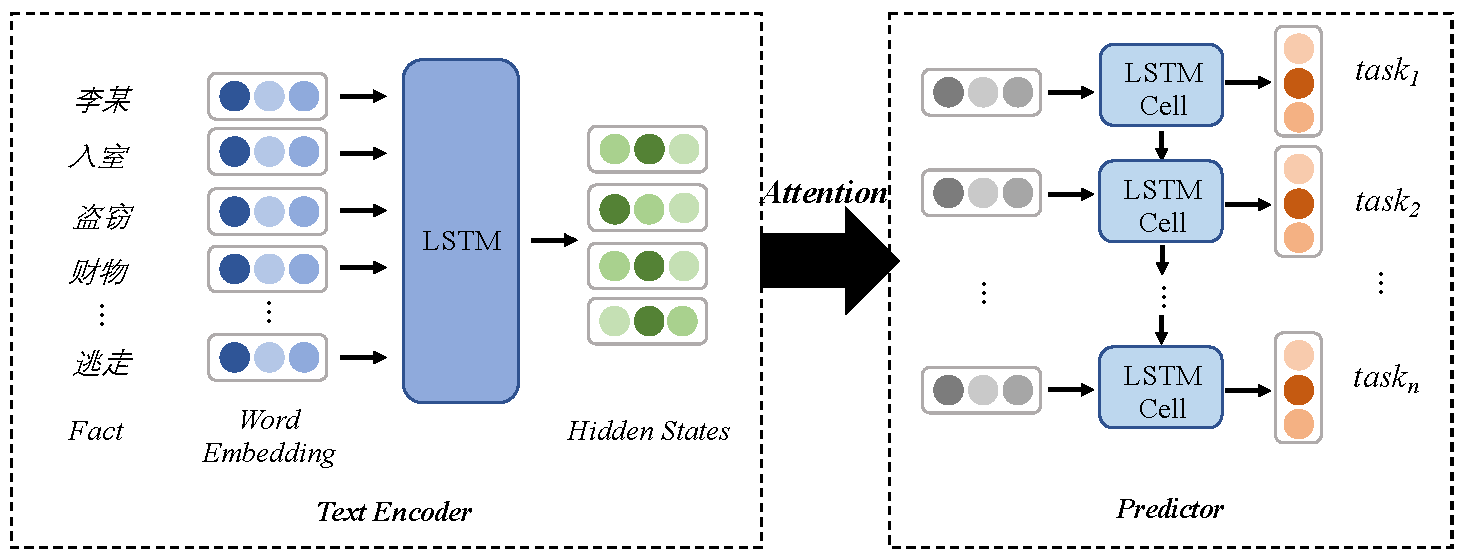
\includegraphics[width=\linewidth]{figures/model1}
    \caption{判决预测模型示意图}
    \label{fig:model1}
\end{figure*}

\subsection{算法模型}
算法使用了LSTM作为模型的编码器,使用了全连接神经网络作为输出层。利用了多任务学习的框架,将多个任务进行联合训练得到了效果的提升。

我们在获得案情文本后,可将算法分为以下几步:
\begin{itemize}
	\item \textbf{输入层}:文本分词与词向量映射。通过上文提到的THULAC与FastText完成本步,将文章映射成词向量序列。
	\item \textbf{编码层}:我们利用了LSTM循环神经网络对词向量序列进行编码,得到一个隐向量序列。之后,我们利用了self-attention机制,来获得对应于不同任务的文本信息。
	\item \textbf{预测层}:我们利用了LSTM Cell来捕获不同任务之间的依赖关系,将不同的任务获得的文本向量当做一个序列,使得任务之间可以获取相应被依赖任务的信息,从而提升相应的效果。
	\item \textbf{输出层}:最后,我们应用了全连接神经网络,将包含任务信息的向量映射到相应的分类中。
\end{itemize}


\section{关键词抽取}
\subsection{任务描述}
在该模块中,我们利用了序列标注模型实现了对案情文本的关键词抽取。任务输入仍旧为一段案情描述的文本,任务的输出为文本中的某一个或者某一些词语,这些词语与法律词汇高度相关,是用来检索相关案件、法条的重要依据。

例如,对于句子:“被告对{\color{red}火灾}发生是否存在{\color{red}过错},应否对原告的合理损失予以{\color{red}赔偿}”中标红的即为关键词,对于检索相关法律法规:“关于{\color{red}火灾过错}引发事故责任划分与{\color{red}赔偿}…”有很强的指导意义。

本模块我们采用了对句子级别的预料进行训练的方式,我们整理了10000条待标注数据,通过寻找专业人士进行人工标注的方法,获取了相应的待标注的训练数据。

在使用时,我们将对每一个句子进行关键词抽取,通过算法规则将所有句子的关键词进行合并、筛选,得到最终文章级别的关键词。关键词抽取的结果将对后续的相关案例检索提供重要的帮助。

\subsection{创新点}

关键词抽取是自然语言处理中,非常常见的任务。在早期,大多数人们使用的是基于词频等特征的无监督学习算法,例如TextRank、LDA、TFIDF算法。对于法律这样一个特定领域,关键词抽取的结果往往是一些法言法语,相比于开放领域上的关键词抽取,有着更强的规律性。因此,我们将目前效果最好的命名实体识别算法运用至该任务。同时,由于训练是在句子级别的语料上进行训练,我们设计了筛选算法,将在所有句子上的抽取结果进行合并筛选,得到了一个较好的效果。

\subsection{算法模型}

\begin{figure*}[ht]
    \centering
    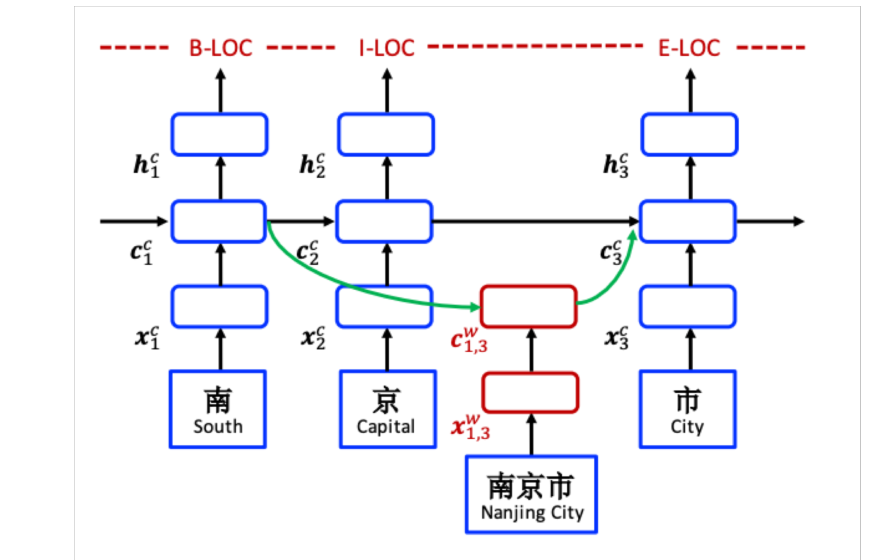
\includegraphics[width=\linewidth]{figures/model2}
    \caption{关键词抽取模型示意图}
    \label{fig:model2}
\end{figure*}

该算法将目前前沿的命名实体识别算法——Lattice LSTM,通过将句子拆分成字级别,对每一个字一个标签,来判断最终关键词的范围。在传统的基于字级别的模型基础上,加入词级别信息,这样克服了字级别信息不足、词级别过度依赖于分词效果的缺陷。

1)	利用n-gram、分词信息等特征为句子中每一个字进行编码,形成字级别特征;

2)	利用好BiLSTM-CRF的框架,通过BiLSTM对字特征进行编码,再通过CRF捕捉序列信息,进行序列标注;

3)	改造字级别的LSTM模型,将字与字之间匹配成的所有的可能词的特征融合到LSTM的信息传递中,得到一个Lattice-word model;

4)	对每个字预测BIE标签,其中B为begin、I为in、E为end;得到最后序列标注的结果。



\section{类案搜索}
\subsection{任务描述}
该模块实现了相关案例推荐的功能。该功能的实现主要基于上述两个模块的模型。该任务模型以案情描述作为输入,通过关键词标签抽取,检索到一批与该案情相似的法律文书,再利用判决预测模块得到的文本向量,对检索到的文书进行重排序,输出一个按照相似度递减的法律文书集合。

\subsection{创新点}
该任务所用算法与传统的搜索引擎算法不同,传统搜索引擎将检索文本与数据库文本进行比对,进而检索出相似度高的文本段。在我们算法中,我们通过抽取出的关键词标签来初步确定相关的文章的集合,再通过判决预测模块中获得的包含文本语义的向量,来对相关集合进行重排序,得到在语义层面相似度最高的文章。

这样的做法改善了传统搜索引擎只关注文本相似度的缺点,通过捕捉语义信息检索以满足用户需求。

\subsection{算法模型}
如上所述,改算法主要分成以下两步:

1)	抽取关键词,利用关键词抽取模块将案情描述中的关键词抽取出来。

2)	利用关键词标签,确定相关文书的集合;将所有关键词与该案情描述关键词一样的案件抽取出来,形成相关文书集合。

3)	相关程度重排序,利用判决预测模块将第2步获得的文书,转化成包含语义信息的文本向量,通过向量的距离来判断文书与输入案情的相关程度,按照相关程度对文书进行重排序。



